\documentclass{beamer}


%\beamertemplateshadingbackground{yellow!100}{white}
\usepackage[bulgarian]{babel}
\usepackage{amsfonts,amsmath}
\usepackage{graphicx}
\usepackage{sansmathaccent}
\pdfmapfile{+sansmathaccent.map}
\usepackage{multirow}
%\usetheme{Warsaw}
\usetheme[secheader]{Madrid}

\usepackage{multimedia}
\logo{
\includegraphics[height=0.5cm]{imi.jpg}}

\newcommand{\be}{\begin{equation}}
\newcommand{\ee}{\end{equation}}
\newcommand{\rf}[1]{(\ref{#1})}
\newcommand{\RR}{\mathbb{R}}
\newtheorem{thm}{Theorem}
\newtheorem{lm}{Lemma}

%\def\ra#1\{\renewcommand{\arraystretch}{#1}
\begin{document}
 %[propagating wave solutions to the 2D BPE]
\title{Числено решение на двумерното Парадигматично уравнение на Бусинеск}

\author{докторант: Красимир Ангелов 
\newline \newline научен ръководител: Наталия Кольковска}
\institute[IMI -- BAS]{Институт по Информатика и Математика\\ Българска Академия на Науките, София, България,\\ e-mail: angelow@math.bas.bg}

%================== frame 01 ======================================
\begin{frame}
\titlepage
\end{frame}

%---------- frame 02 ----------------
\begin{frame}
\tableofcontents 
\setbeamertemplate{table of contents shaded}[default]
\section{Преглед на литературата}
\section{Цели}
\section{Парадигматичното уравнение на Бусинеск - смяна на променливите}
\section{Числени методи за Парадигматичното уравнение на Бусинеск}
\subsection{Консервативна схема}
\subsubsection{Сходимост}
\subsubsection{Запазване на дискретната енергия}
\subsection{Метод на Тейлор и метод на правите}
\subsubsection{Сходимост}
\section{Числени резултати}
\subsection{Дискретна енергия и форма - сравнение между метода на Тейлор и Консервативната схема}
\subsection{Форма и максимум на решението при метода на Тейлор}
\subsection{Числен тест при $\beta = 3, c=0.3$}


%\tableofcontents 
\end{frame}

%---------- frame 03 ----------------
\begin{frame}
\frametitle{Преглед на литературата}

\begin{itemize}
  \item 2010, Christov, C.I., Kolkovska, N., Vasileva, D., On the Numerical Simulation of Un-
steady Solutions for the 2D BPE, {\it In: Numerical Methods and Applications},

  \item 2011, Chertok, A., Christov, C.I., Kurganov, A., Central-Upwind Schemes for the BPEs,
{\it Computational Science and High Performance Computing IV},

  \item 2012, Kolkovska, N., Angelow K., A Multicomponent Alternating Direction Method for Numerical Solving of Boussinesq Paradigm Equation, {\it In:  I. Dimov, I., Farago, I., Vulkov, L. (eds.) NAA},
  
  \item 2013, Dimova M., Vasileva D., Comparison of Two Numerical Approaches to Boussinesq Paradigm Equation,  {\it Lect. Notes Comput. Sci.}, 
  
  \item 2022, Yuyu He, Hongtao Chen, Efficient algorithm and convergence analysis of conservative SAV compact difference scheme for Boussinesq Paradigm equation, {\it Computers and Mathematics with Applications}
\end{itemize}

\end{frame}

%---------- frame 04 ----------------

\begin{frame}
\frametitle{Цели}

\begin{itemize}
  \item да се построи числен метод (на Тейлор), който използва диференчни схеми с висок (втори, четвърти и шести) ред на апроксимация, за решението на ПУБ,
  
     \item да се изследват следните свойства на ПУБ при по-високи скорости близки до допустимия максимум $c \approx c_{max}$, $c < c_{max}$
  \begin{itemize}
     \item енергия,
     \item форма,
     \item максимум,     
  \end{itemize}
	използвайки началното условие получено от елиптичната задача, където $c_{max} = \min (1/ \sqrt{\beta_1},1)$,

  \item да се сравнят числените резултати получени с метода на Тейлор и Консервативната схема при $O(h^2)$
    
\end{itemize}


\end{frame}

%---------- frame 05 ----------------

\begin{frame}
\frametitle{Публикации}

Резултатите от численото решение на двумерните стационарно и хиперболични уравнения на Бусинеск са
публикувани в
\begin{itemize}
  \item K. Angelow, N. Kolkovska, Numerical Study of Traveling Wave Solutions to 2D BE, {\it Serdica Journal of Computing},
  \item K. Angelow, New Boundary Condition for the Two Dimensional Stationary Boussinesq Paradigm Equation, {\it International Journal of Applied Mathematics},
   \item K. Angelow, Comparison Between Two Numerical Methods for Solution of 2D BPE, {\it AIP Conference Proceedings}
\end{itemize}

\end{frame}

%---------- frame 06 ----------------

\begin{frame}
\frametitle{Парадигматичното уравнение на Бусинеск - смяна на променливите}

\begin{align}
&u_{tt} - \Delta u -\beta_1  \Delta u_{tt} +\beta_2 \Delta ^2 u + \Delta f(u)=0, \, t\in\RR^+,\label{eq1}
\\
&f(u) = u^2 \nonumber \\  \nonumber &u(x,y,0)=u_0(x,y), \, u_t(x,y,0)=u_1(x,y)  , 
\\  &u(x,y) \rightarrow 0, \,  \Delta u(x,y) \rightarrow 0 ,  \quad \text{при} \sqrt{x^2 + y^2} \rightarrow \infty, \label{eq11} 
\end{align}

\end{frame}

%---------- frame 07 ----------------

\begin{frame}
\frametitle{Парадигматичното уравнение на Бусинеск - смяна на променливите}
Следната смяна на променливите 
\begin{align}
x = \sqrt{\beta_1} \bar{x}, \quad y = \sqrt{\beta_1} \bar{y}, \quad t = \sqrt{\beta_1} \bar{t}
\end{align}

трансформира \rf{eq1} в

\be\label{problemVC}
\beta(I-\Delta) \frac{\partial^2 u}{\partial t^2}=
  \Delta u -\Delta^2 u +\Delta(-\alpha \beta u^2 + (\beta - 1 )u)
\ee

където $\beta = \beta_1/\beta_2$.

\end{frame}



%---------- frame 08 ----------------
\begin{frame}
\frametitle{Запазване на енергията}
\framesubtitle{Енергията за непрекъснатата задача \rf{problemVC}}
\begin{align}\label{ex-en}
E(u(t)) = E(u(0)) =&\int_{R^2} u_t \left((A^{-1}+E)u_t\right) dxdy+
\beta \int_{R^2} u^2 dxdy \nonumber\\
+& \int_{R^2}u \left(A u\right) dxdy
-\frac{2 \alpha \beta}{3} \int_{R^2} u^3 dxdy =const.
\end{align}
$E(u(t))$ представлява аналитичeн израз за енергията от уравнението \rf{problemVC}, където $Au=-\Delta u$.
\end{frame}

%------------------------ frame 09 -----------------------------------------

\begin{frame}
\frametitle{Изчислителна област $\Omega_h$}
\framesubtitle{Равномерна мрежа $h=(h_1, h_2)$}
\begin{center}\vspace{0.4cm}
	\begin{minipage}[b]{0.6\linewidth}
		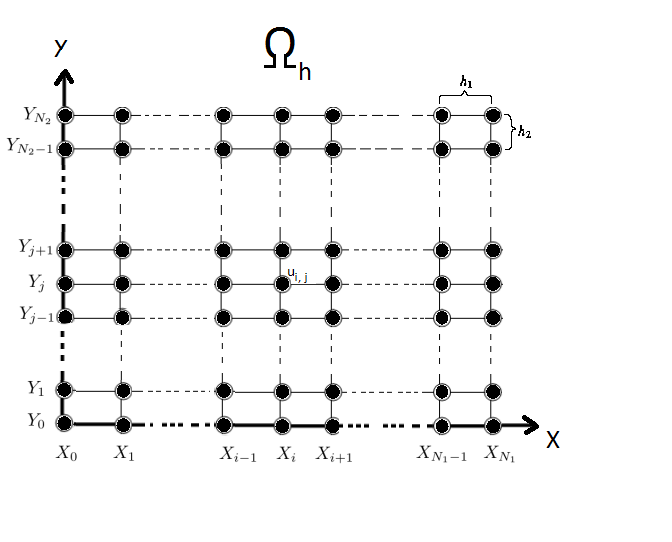
\includegraphics[width=\linewidth]{Omega_dah.png}
	\end{minipage}
\end{center}

\end{frame}

%---------- frame 10 ----------------

\begin{frame}
\frametitle{Консервативна схема}
\framesubtitle{Дискретизация на вторите производни}
Апроксимацията на вторите производни се дефинира чрез:
\begin{equation}
\frac{\partial^2 u}{\partial t^2}(x_i, y_j, t_k ) = \frac{ u^{(k+1)}_{i, j} - 2u^{(k)}_{i,j} + u^{(k-1)}_{i,j} }{\tau^2} + O(\tau^2) 
\end{equation}

\begin{equation}
\frac{\partial^2 u}{\partial x^2}(x_i, y_j, t_k ) = \frac{ u^{(k)}_{i+1, j} - 2u^{(k)}_{i,j} + u^{(k)}_{i-1,j} }{h_1^2} + O(h_1^2) 
\end{equation}

\begin{equation}
\frac{\partial^2 u}{\partial y^2}(x_i, y_j, t_k ) = \frac{ u^{(k)}_{i, j+1} - 2u^{(k)}_{i,j} + u^{(k)}_{i,j-1} }{h_2^2} + O(h_2^2) 
\end{equation}


\begin{equation}
\Delta_h u(x_i, y_j, t_k )  = \frac{ u^{(k)}_{i+1, j} - 2u^{(k)}_{i,j} + u^{(k)}_{i-1,j} }{h_1^2} + \frac{ u^{(k)}_{i, j+1} - 2u^{(k)}_{i,j} + u^{(k)}_{i,j-1} }{h_2^2}
\end{equation}

\end{frame}

%------------------------ frame 11 -----------------------------------------

\begin{frame}
\frametitle{Консервативна схема}
\framesubtitle{Диференчно уравнение}
Диференчно уравнение с апроксимация от втори ред за \rf{problemVC}:
\begin{equation}\label{problemVCDiscrete}
\beta (I-\Delta_h)\frac{ u^{(k+1)}_{i, j} - 2u^{(k)}_{i,j} + u^{(k-1)}_{i,j} }{\tau^2} = (\Delta_h - \Delta_h^2)u^{(k)}_{i,j} + \Delta_h(g(u^{(k)}_{i,j}))
\end{equation}
%
където нелинейния член $g$ е дефиниран чрез:
\begin{align}
g(u^{(k)}_{i,j})=& -\frac{\alpha \beta} { 3 } \left( (u^{(k+1)}_{i,j})^2 + (u^{(k-1)}_{i,j})(u^{(k+1)}_{i,j}) + (u^{(k-1)}_{i,j})^2 \right) + \nonumber\\
+&\frac{ (\beta - 1 )}{ 2 }\left( u^{(k+1)}_{i,j} + u^{(k-1)}_{i,j} \right).
\end{align}


\end{frame}


%------------------------ frame 12 -----------------------------------------

\begin{frame}
%C
\frametitle{Консервативна схема}
\framesubtitle{Сходимост}
$T = 10$
\begin{table}[ht]
\centering
\small
		\begin{tabular}{||c|l|ll|ll||}
			\hline
			\hline
      \multirow{2  }{*}{ }        & \multirow{2  }{*}{$h$, $\tau$}  & \multirow{2  }{*}{грешки $\Vert E_i\Vert_{L_2}$}  &ред на& \multirow{2  }{*}{грешки $\Vert E_i\Vert_{L_\infty}$}  &ред на  \\
	                                        &                                                     &                                                                 &  сход. &                                                                       & сход. \\
   			\hline 
					\hline 
  $\beta=3$                &0.2, 0.1         &                    &                &                  &                   \\
   c=0.45                     &0.1, 0.05         & 1.006740   &                & 1.059568 &                   \\
     $O(h^2 + \tau^ 2)$ &0.05, 0.025  &0.358090    	& 1.50       	& 0.368755   &   1.52   \\
	   \hline
			\hline 
       $\beta=1$           & 0.4, 0.2       &                   &           &                 &   \\
                  c=0.9       & 0.2, 0.1        & 0.124597   &          &0.048148  &   \\
  $O(h^2+ \tau^2)$  & 0.1, 0.05       & 0.028320   & 2.14  &0.012227  & 1.98 \\
	   \hline
			\hline 
		\end{tabular}
		\caption{Тест на Рунге за сходимост при Консервативната схема с нулево гранично условие и грешки от апроксимацията $O(h^{2} + \tau^2 )$. Грешките $E_i$ са изчислени в $L_2$ и $L_\infty$ норми.}
\label{tableC}
\end{table}

\end{frame}

%------------------------ frame 13 -----------------------------------------

\begin{frame}

\frametitle{Консервативна схема}
\framesubtitle{Енергията за дискретното диференчно уравнение \rf{problemVCDiscrete}}

\begin{figure}[ht]\vspace{0.02cm}
	\begin{minipage}[b]{0.48\linewidth}
		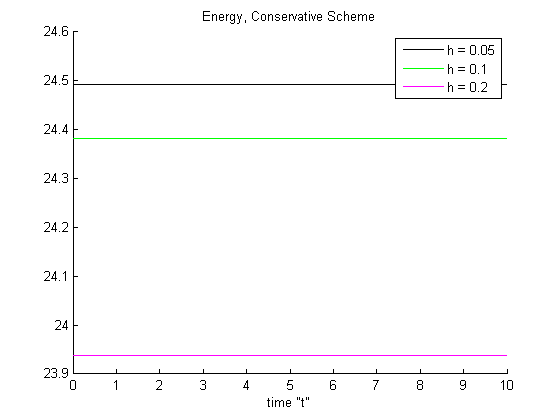
\includegraphics[width=\linewidth]{../amitans/figures/Energy_EnergySave_bt3_c045_x3O.png}	
	\end{minipage}
	\begin{minipage}[b]{0.48\linewidth}
		 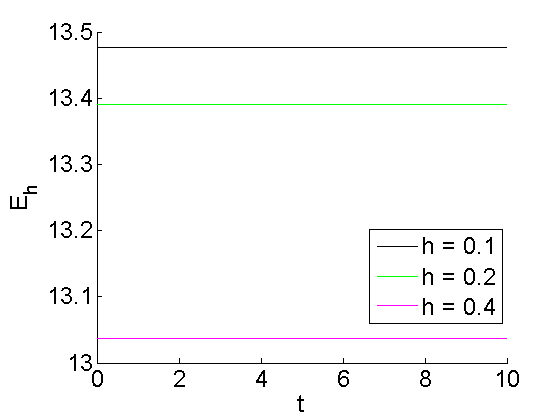
\includegraphics[width=\linewidth]{../amitans/figures/Energy_EnergySave_bt1_c090_x3O.png}
	\end{minipage}
\caption{Дискретната енергия ot Консервативната схема при $\beta=3,c=0.45$ (ляво) и $\beta=1,c=0.9$ (дясно) с апроксимационна грешка $O(|h|^2 + \tau^2)$ във времето $T_{\tau} = [0, 10]$.}
\label{EnOnly}
\end{figure}

\end{frame}

%------------------------- frame 14 -----------------------------------------

\begin{frame}
\frametitle{Метод на Тейлор и метод на линиите за ПУБ}
\begin{center}\vspace{0.25cm}
	\begin{minipage}[b]{0.45\linewidth}
		 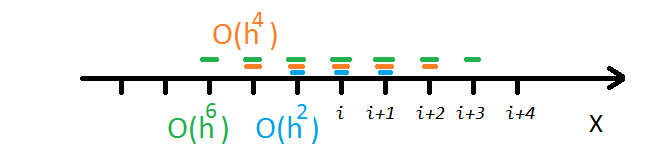
\includegraphics[width=\linewidth]{../amitans/figures/FDS.png}
	\end{minipage}	
\end{center}
Нека $u_{i,j}(t)$ е апроксимацията на $u(x_i, y_j, t)$ в точка от мрежата $(x_i, y_j)$.
\\
Нека $\Delta_{h,p} u_{i,j}$ е диференчния оператор, който апроксимира $\Delta u$ с грешкa $O(|h|^p)$ (p=2, 4, 6).
\\
%here99
От \rf{problemVC} се получава следната система от ОДУ:
\be \label{DiscreteEq}
\beta (I-\Delta_{h,p}) \frac{\partial^2 u}{\partial t^2}(x_i, y_j, t)=
 (\Delta_{h,p} - \Delta_{h,p}^2) u_{i, j}(t) + \Delta_{h,p} ( ( u_{i, j}(t) )^2 )
\ee
за $i = 0..N_1$ и $j=0..N_2$. За всяко ОДУ от системата е направено развитие в ред на Тейлор:
\begin{align} \label{TSe}
u(x_i, y_j, t+\tau) = u(x_i, y_j, t) + \tau \frac{ \partial u }{ \partial t }(x_i, y_j, t)  + ... 
%\nonumber
%\\
\frac{ \tau^p }{ p! } \frac{ \partial^p u }{ \partial t^p }(x_i, y_j, t) + O(\tau^{p+1})
\end{align}

\end{frame}

%---------------------------- frame 15 --------------------------------------

\begin{frame}
\frametitle{Mетод на Тейлор и метод на линиите за ПУБ}
\framesubtitle{Изчисляване на реда на Тейлор \rf{TSe}}
\begin{itemize}
 \item Нач. Условие $\rightarrow$ $u(x_i, y_j, t=0)$, $\frac{ \partial u }{ \partial t }(x_i, y_j, t=0)$,
 \item \rf{DiscreteEq} $\rightarrow$ $\frac{ \partial^2 u }{ \partial t^2 }(x_i, y_j, t=0)$ ,
 \item Диференциране на уравнение $\frac{ \partial^{p-2} u }{ \partial t^{p-2} }$ \rf{DiscreteEq} $\rightarrow$  $\frac{ \partial^p u }{ \partial t^p }(x_i, y_j, t)$,
 \item Заместване на изчислените производни в реда на Тейлор \rf{TSe}.
\end{itemize}


Така се получават следните апроксимации
\begin{description}
 \item[$p=2$] $O(|h|^2 + \tau^2)$,
 \item[$p=4$] $O(|h|^4 + \tau^4)$,
 \item[$p=6$] $O(|h|^6 + \tau^6)$.
\end{description}

\end{frame}

%---------------------------- frame 16 --------------------------------------

\begin{frame}
\frametitle{Метод на Тейлор и метод на линиите за ПУБ}
\framesubtitle{Сходимост}

\begin{table}[ht]
\centering
\small
\resizebox{0.6\linewidth}{!}{%
		\begin{tabular}{||c|l|ll|ll||}
			\hline
			\hline
      \multirow{2  }{*}{ $T = 10$ }        & \multirow{2  }{*}{$h$, $\tau$}  & \multirow{2  }{*}{грешки $\Vert E_i \Vert_{L_2}$ } &ред на& \multirow{2  }{*}{грешки $\Vert E_i \Vert_{L_\infty}$}  &ред на  \\
	         &                    &                               & сход   &                                        & сход. \\
\hline 
\hline 
  $\beta=3$               &0.2, 0.1      &              	&           &                	&      \\
   c=0.45                   &0.1, 0.05    &0.968044  	&           &1.034208   &       \\
 $O(h^2 + \tau^ 2)$ 	&0.05, 0.025	& 0.340955 	& 1.51    &0.351518  	&  1.56      \\
\hline 
  $\beta=3$               &0.2, 0.1      &              	&          	&                 &      \\
   c=0.45                   &0.1, 0.05    &0.191389 	&          	&0.194056   	&       \\
$O(h^4+ \tau^4)$	&0.05, 0.025	&0.013036 	& 3.88   	&0.013664   	& 3.83       \\
\hline 
  $\beta=3$               &0.2, 0.01    &                	&          	&                 &      \\
     c=0.45                 &0.1, 0.05    &0.032671 	&          	& 0.033625  	&       \\
  $O(h^6+ \tau^6)$ 	&0.05, 0.025	&0.000599 	&5.78    	& 0.000635  	& 5.73       \\
\hline
\hline 
       $\beta=1$        	&0.4, 0.2      &             	&            &           &   \\
           c=0.9    		&0.2, 0.1      &  0.148014 	&            &0.058905 &   \\
  $O(h^2+ \tau^2)$  	&0.1, 0.05   	& 0.030690  	&2.27  	 &0.014185   & 2.05 \\
\hline
      $\beta=1$           &0.4, 0.2    	&            	&               &             &    \\
       c=0.9                 &0.2, 0.1     & 0.028869   &        &  0.013791   &   \\
 $O(h^4+ \tau^4)$ 	&0.1, 0.05   	&0.001860 	& 3.96  & 0.000996  & 3.80  \\
\hline
  $\beta=1$     		&0.4, 0.2   	&            	&          	&                  &      \\
      c=0.9                  &0.2, 0.1   	&0.006732 	&            & 0.003334      &       \\
 $O(h^6+ \tau^6)$ 	&0.1, 0.05 	& 0.000249 	& 4.75 	& 0.000068  & 5.61        \\
\hline
\hline 
		\end{tabular}
		}%
		\caption{Скорост на сходимост на численото решение при метода на Тейлор с нулево гранично условие и грешки от апроксимацията $O(h^{2} + \tau^2 )$, $O(h^{4} + \tau^4 )$ и $O(h^{6} + \tau^6 )$. Грешките $\bar E_i$ са измерени в $L_2$ и $L_\infty$ норми.}
\label{table:A}
\end{table}

\end{frame}

%----------------------------- frame 17 -------------------------------------

\begin{frame}
\frametitle{Числени резултати}
\framesubtitle{Параметри}

Дисперсионен параметър $\beta$, скорост $c$, време $T$ и големина на областта
\begin{description}
 \item[Тест 1] $\beta = 3$, $c = 0.45$, $\Omega = [-30, 30] \times [-27, 27]$, $T = 10$
 \item[Тест 2] $\beta = 1$, $c = 0.9$, $\Omega = [-128, 128] \times [-58, 58]$, $T = 10$
\end{description}

Ред на апроксимация $p$
\begin{enumerate}
  \item Conservative FDS with $O(|h|^2 + \tau^2)$
  \item TS method with $O(|h|^p + \tau^p)$ and $p = 2, 4, 6$
\end{enumerate}

Тест 1 and Тест 2 използват нулево гранично условие - по границата на областта се използват несиметрични крайни разлики със същия ред на апроксимация $p$ използван във вътрешността на областта $\Omega_h$.
\end{frame}

%---------------------------------- frame 18 --------------------------------

\begin{frame}
\frametitle{Числени резултати}
\framesubtitle{Дискретна енергия - сравнение между метода на Тейлор и Консервативната схема}

\begin{center}\vspace{0.4cm}
	\begin{minipage}[b]{0.49\linewidth}
		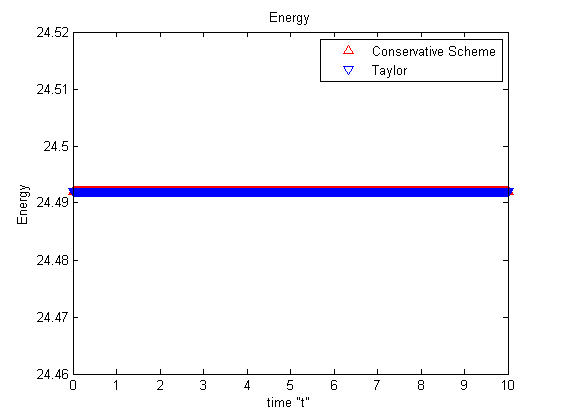
\includegraphics[width=\linewidth]{../amitans/figures/Energy_bt3_c045_h005.png}
	\end{minipage}	
	\begin{minipage}[b]{0.49\linewidth}
		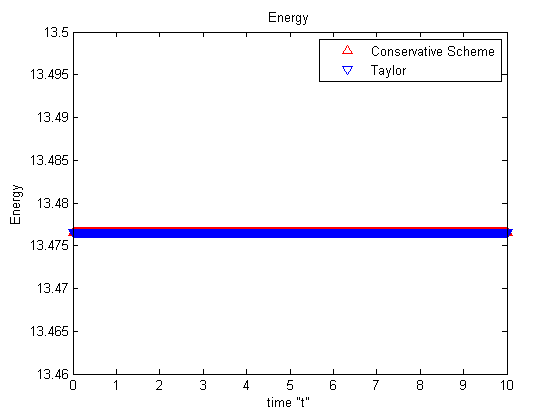
\includegraphics[width=\linewidth]{../amitans/figures/Energy_bt1_c090_h010.png}
		
	\end{minipage}
\end{center}
Дискретната енергия като функция на времето до $T = 10$ при Тест 1 (ляво) и Тест 2 (дясно) и апроксимация $O(|h|^2 + \tau^2)$.
\end{frame}


%---------------------------------- frame 19 --------------------------------

\begin{frame}
\frametitle{Числени резултати}
\framesubtitle{Форма - сравнение между метода на Тейлор и Консервативната схема при $\beta = 3, c=0.45$}
\begin{center}\vspace{0.4cm}
	\begin{minipage}[b]{0.32\linewidth}
		 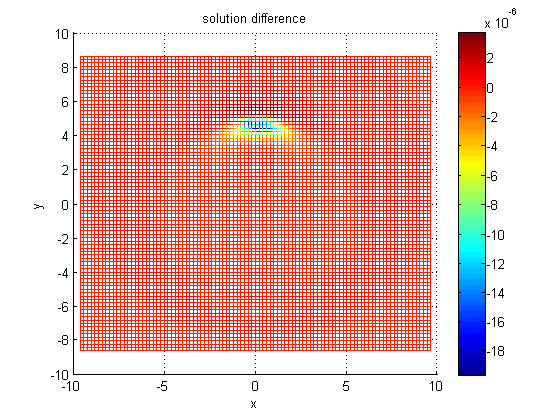
\includegraphics[width=\linewidth]{../amitans/figures/compare_30_bt3_c045_h020.png}
	\end{minipage}	
	\begin{minipage}[b]{0.32\linewidth}
		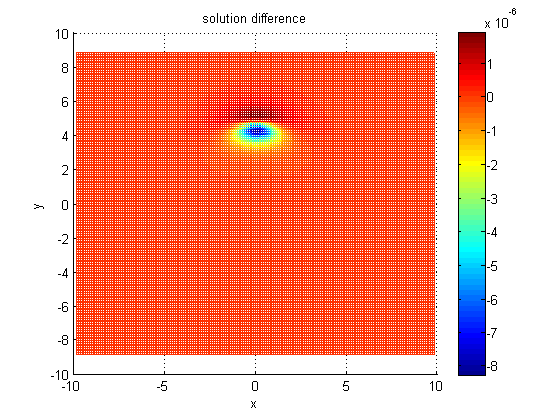
\includegraphics[width=\linewidth]{../amitans/figures/compare_30_bt3_c045_h010.png}
	\end{minipage}	
	\begin{minipage}[b]{0.32\linewidth}		
		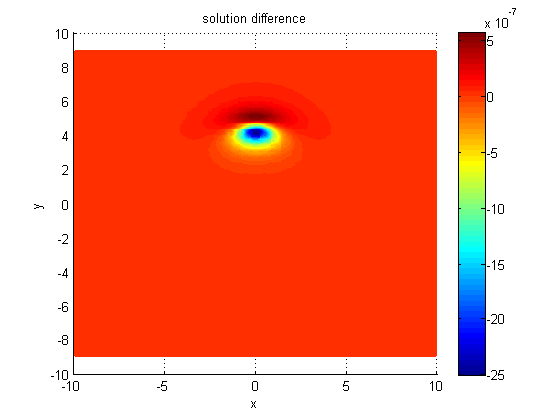
\includegraphics[width=\linewidth]{../amitans/figures/compare_30_bt3_c045_h005.png}
	\end{minipage}
\end{center}
Разликите в числените решения получени с метода на Тейлор и Консервативната схема за време $T=10$ и апроксимация $O(|h|^2 + \tau^2)$ за Тест 1. От ляво на дясно $h=0.2, 0.1, 0.05$. Графиката представлява само една девета от цялата област $\Omega_h$.
\end{frame}

%---------------------------------- frame 20 --------------------------------

\begin{frame}
\frametitle{Числени резултати}
\framesubtitle{Форма - сравнение между метода на Тейлор и Консервативната схема при $\beta = 1, c=0.9$}
\begin{center}\vspace{0.4cm}
	\begin{minipage}[b]{0.32\linewidth}
		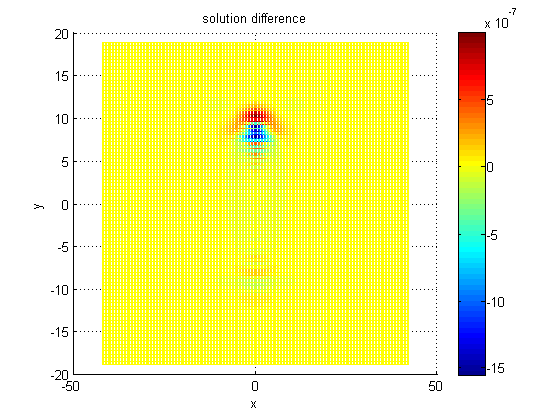
\includegraphics[width=\linewidth]{../amitans/figures/compare_128_bt1_c09_h040.png}
	\end{minipage}	
	\begin{minipage}[b]{0.32\linewidth}
		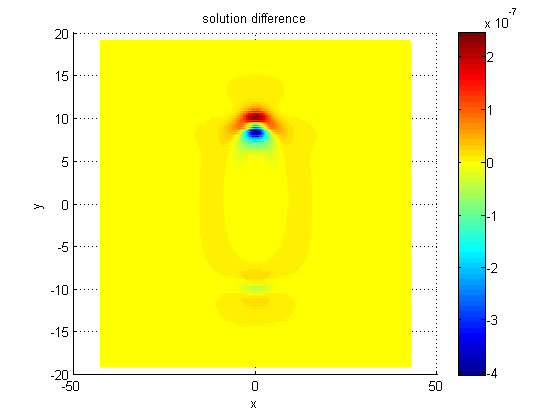
\includegraphics[width=\linewidth]{../amitans/figures/compare_128_bt1_c09_h020.png}
	\end{minipage}	
	\begin{minipage}[b]{0.32\linewidth}
		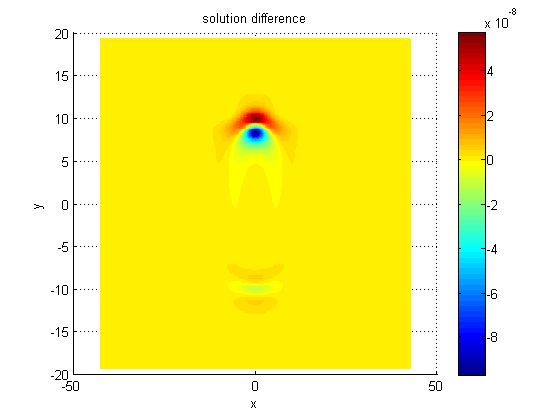
\includegraphics[width=\linewidth]{../amitans/figures/compare_128_bt1_c09_h010.png}		 
	\end{minipage}
\end{center}
Разликите в числените решения получени с метода на Тейлор и Консервативната схема за време $T=10$ и апроксимация $O(|h|^2 + \tau^2)$ за Тест 1. От ляво на дясно $h=0.4, 0.2, 0.1$. Графиката представлява само една девета от цялата област $\Omega_h$.
\end{frame}

%---------------------------------- frame 21 --------------------------------

\begin{frame}
\frametitle{Числени резултати}
\framesubtitle{Максимума на решението при метода на Тейлор, $p=2,4,6$ и $T=10$}

\begin{figure}[ht]
	\centering
	\begin{minipage}[b]{0.4\linewidth}
		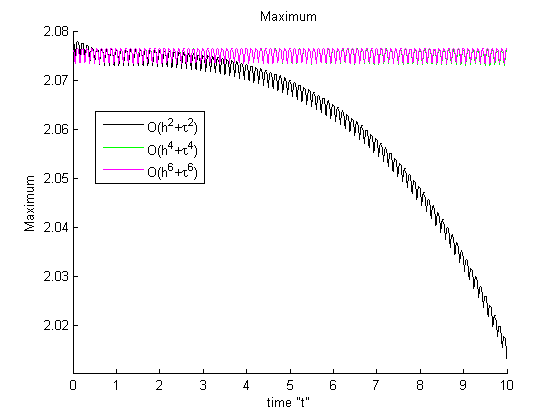
\includegraphics[width=\linewidth]{../amitans/figures/maximum_30_bt3_c045_h005.png}
	\end{minipage}	
	\begin{minipage}[b]{0.4\linewidth}
		 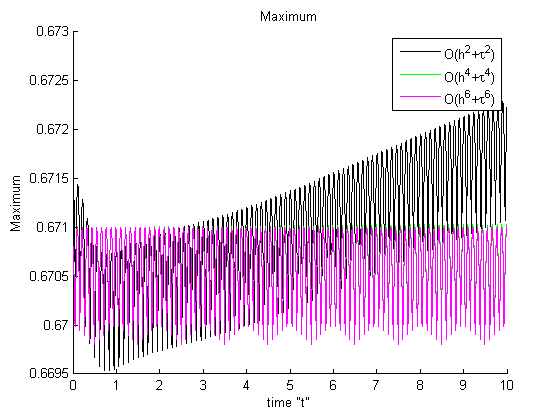
\includegraphics[width=\linewidth]{../amitans/figures/maximum_128_bt1_c090_h010.png}
	\end{minipage}

Развитието на максимума за време $T=10$, $\tau = h/100$, при Тест 1 (ляво) и Тест 2 (дясно) .
\end{figure}

\end{frame}

%---------------------------------- frame 22 --------------------------------

\begin{frame}
\frametitle{Числени резултати}
\framesubtitle{Максимума на решението при метода на Тейлор и $T=30$}

\begin{figure}[ht]
	\centering
	\begin{minipage}[b]{0.40\linewidth}
		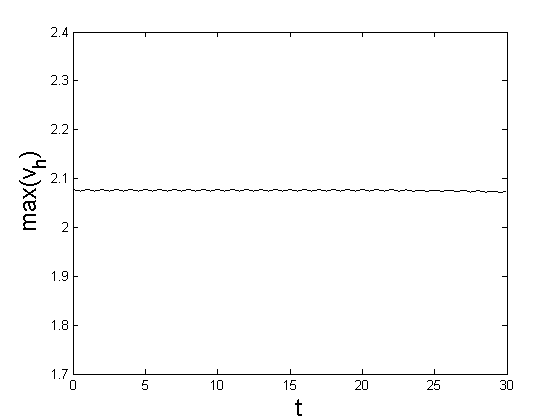
\includegraphics[width=\linewidth]{../amitans/figures/maximum_30_T30_bt3_c045_h005.png}
	\end{minipage}	
	\begin{minipage}[b]{0.40\linewidth}
		 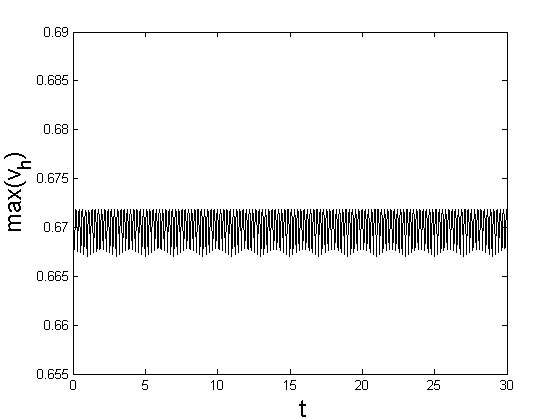
\includegraphics[width=\linewidth]{../amitans/figures/maximum_30_T30_bt1_c090_h020.png}
	\end{minipage}
\caption{Максимума на решението върху по-голям интервал от време $[0, 30]$ при Тест 1 (ляв панел) и Тест 2 (десен панел). Използвана е апроксимация от шести ред $p=6$ със стъпки $h=0.05$, $\tau = 0.001$ при Тест 1 и $h=0.2$,  $\tau=0.02$ при Тест 2.}
\end{figure}

\end{frame}

%---------------------------------- frame 23 --------------------------------

\begin{frame}
\frametitle{Числени резултати}
\framesubtitle{Форма на решението при метода на Тейлор}

\begin{table}[ht]
\centering
\small
\resizebox{8cm}{!}{
		\begin{tabular}{||c|l|l|l||}
			\hline
			\hline
                  & $h$, $\tau$  & $||u^{(0)} - u^{(N_t)}||_{L_2}$  & $||u^{(0)} - u^{(N_t)}||_{L_\infty}$   \\
   		\hline 
			\hline
  $\beta=3$                &0.2, 0.001            & 1.494351 & 1.533173    \\
   c=0.45                     &0.1, 0.0005          & 0.466991 & 0.484011       \\
     $O(h^2 + \tau^ 2)$ &0.05, 0.00025   & 0.127641 & 0.132504      \\
			\hline 
  $\beta=3$               &0.2, 0.02       &0.220560 & 0.230486       \\
   c=0.45                    &0.1, 0.01      &0.013762 & 0.014391        \\
     $O(h^4+ \tau^4)$ &0.05, 0.005&0.000877 & 0.000917         \\
			\hline 
  $\beta=3$               &0.2, 0.02        &  0.035965 & 0.038039        \\
     c=0.45                 &0.1, 0.01        &0.000600 & 0.000633       \\
     $O(h^6+ \tau^6)$ &0.05, 0.005 &0.000010 & 0.000010          \\
	   \hline
			\hline 
       $\beta=1$       &0.4, 0.002        & 0.244208 & 0.103833 \\
                  c=0.9    &0.2, 0.001       &  0.057175 & 0.026919  \\
  $O(h^2+ \tau^2)$ &0.1, 0.0005   & 0.013938 & 0.006622  \\
			\hline
      $\beta=1$               &0.4, 0.04     &0.028546 & 0.012203 \\
       c=0.9                     &0.2, 0.02     & 0.001757 & 0.000958     \\
       $O(h^4+ \tau^4)$ &0.1, 0.01   & 0.000112 & 0.000061   \\
    \hline
  $\beta=1$                  &0.4, 0.04    &0.006415 & 0.002792  \\
      c=0.9                    &0.2, 0.02   &0.000112 & 0.000065     \\
     $O(h^6+ \tau^6)$ &0.1, 0.01 & 0.000002 & 0.000001         \\
	   \hline
			\hline 
		\end{tabular}
		}
		
\end{table}
Разликата между началния $t=0$ и крайния $t=10$ моменти от време.
\end{frame}

%------------------------------------------------------------------

\begin{frame}
\frametitle{Conclusion}

\begin{description}
 \item[-] 2D BPE is solved using TS method with high approximation orders $O(|h|^k+\tau^k)$, $k=2,4,6$
 \item[-] the results are compared with the Conservative Scheme for $O(|h|^2+\tau^2)$
 \item[-] the Energy of the TS solution is saved with high accuracy over the time interval $[0, 10]$
 \item[-] the numerical solutions for wave speeds near the upper limit $c_{max} = min\{1, \sqrt{\beta_2/\beta_1} \}$ are stable in form and their maximums change with small errors over the time interval $[0, 10]$.
\item[-] the obtained solutions show soliton behavior!
\end{description}

\end{frame}

%------------------------------------------------------------------

\begin{frame}
\frametitle{Wave Evolution}
\begin{center}\vspace{0.4cm}
	\begin{minipage}[b]{0.30\linewidth}
		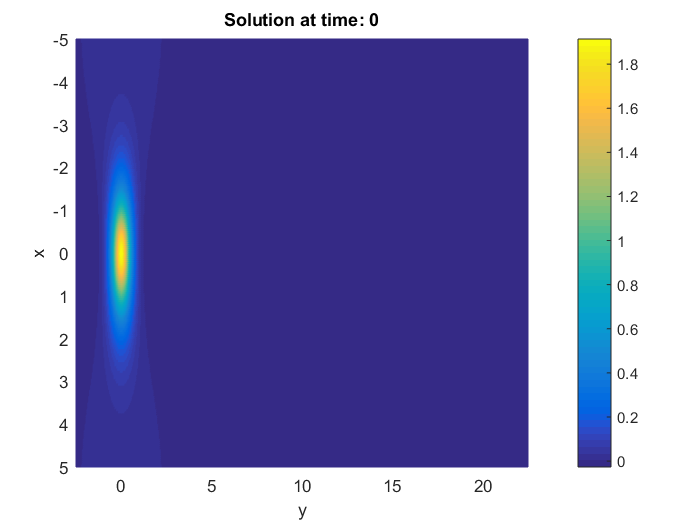
\includegraphics[width=\linewidth]{../amitans/figures/Solution_bt3_t=0.png}
	\end{minipage}	
	\begin{minipage}[b]{0.30\linewidth}
		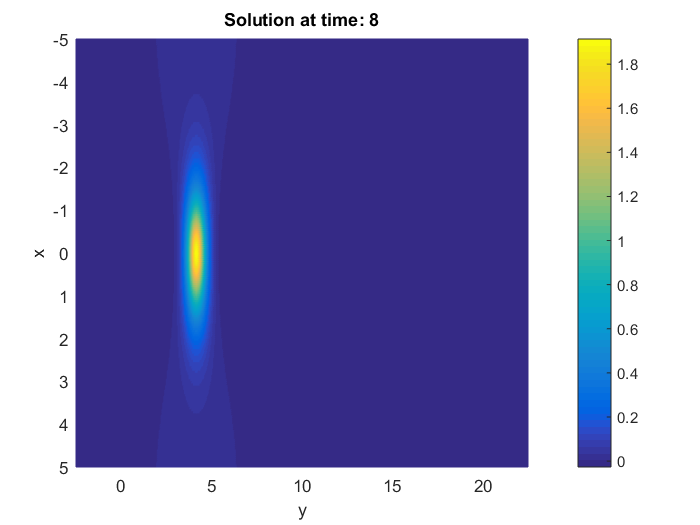
\includegraphics[width=\linewidth]{../amitans/figures/Solution_bt3_t=8.png}
	\end{minipage}	
	\begin{minipage}[b]{0.30\linewidth}
		 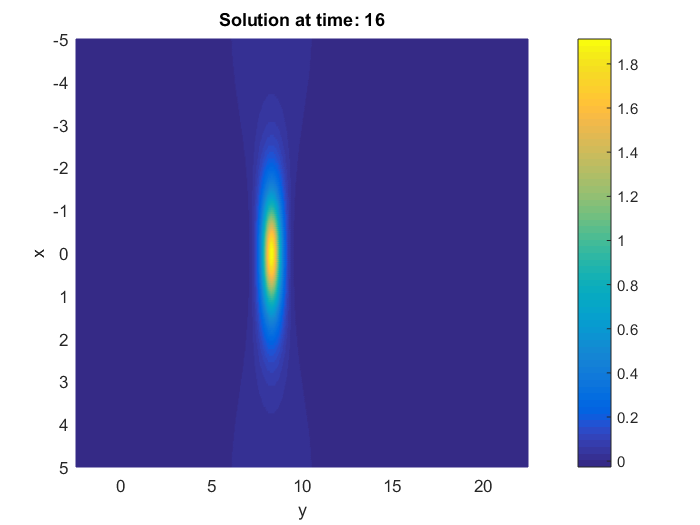
\includegraphics[width=\linewidth]{../amitans/figures/Solution_bt3_t=16.png}
	\end{minipage}
	\begin{minipage}[b]{0.30\linewidth}
		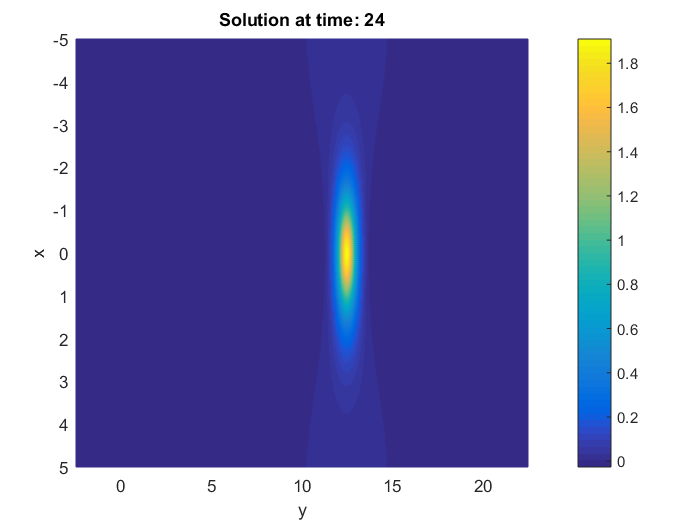
\includegraphics[width=\linewidth]{../amitans/figures/Solution_bt3_t=24.png}
	\end{minipage}	
	\begin{minipage}[b]{0.30\linewidth}
		 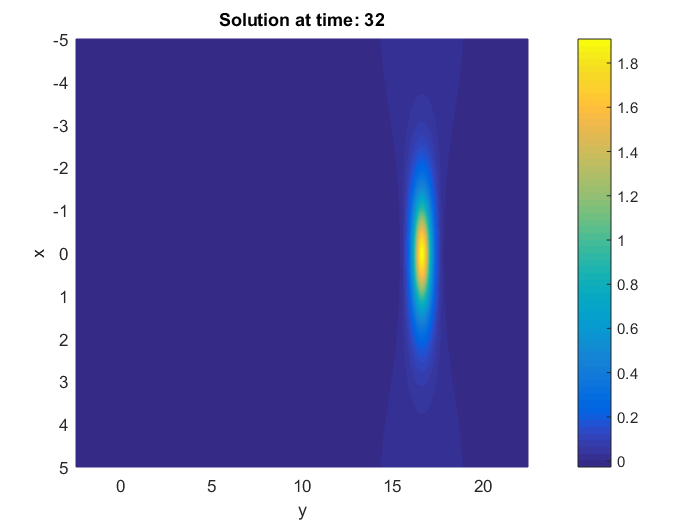
\includegraphics[width=\linewidth]{../amitans/figures/Solution_bt3_t=32.png}
	\end{minipage}
	\begin{minipage}[b]{0.30\linewidth}
		 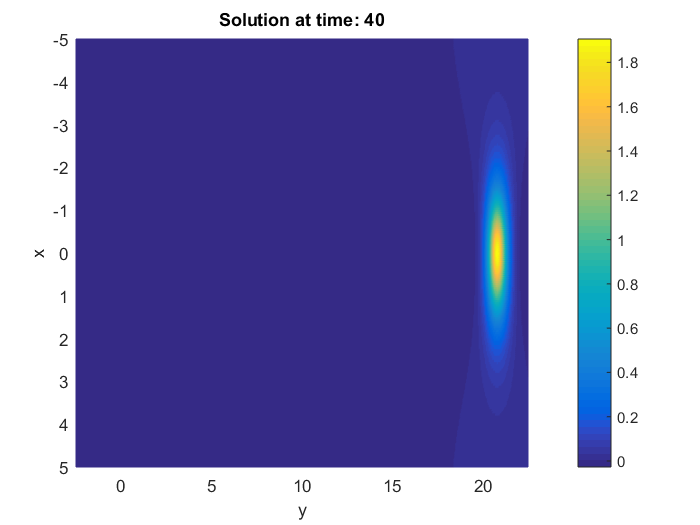
\includegraphics[width=\linewidth]{../amitans/figures/Solution_bt3_t=40.png}
	\end{minipage}
\end{center}
Numerical solution of single wave for $\beta=3$ and $c = 0.52$ at times $t=0,8,16,24,32,40$.
\end{frame}

%------------------------------------------------------------------

\begin{frame}
\frametitle{Wave Evolution}
\begin{center}\vspace{0.4cm}
	\begin{minipage}[b]{0.30\linewidth}
		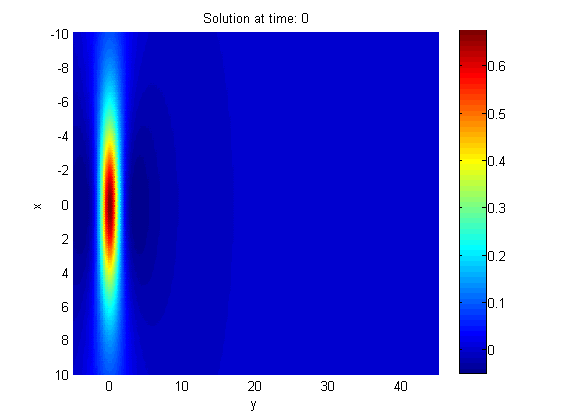
\includegraphics[width=\linewidth]{../amitans/figures/Solution1_t=0.png}
	\end{minipage}	
	\begin{minipage}[b]{0.30\linewidth}
		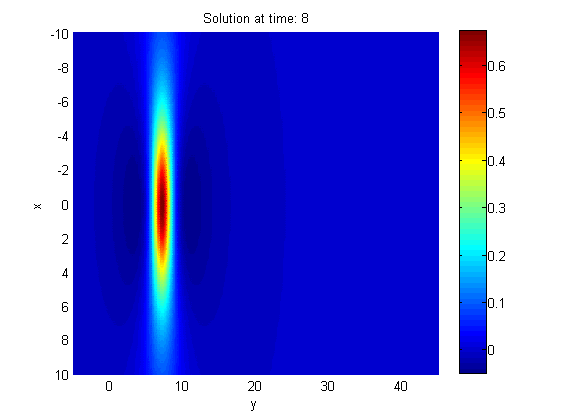
\includegraphics[width=\linewidth]{../amitans/figures/Solution1_t=8.png}
	\end{minipage}	
	\begin{minipage}[b]{0.30\linewidth}
		 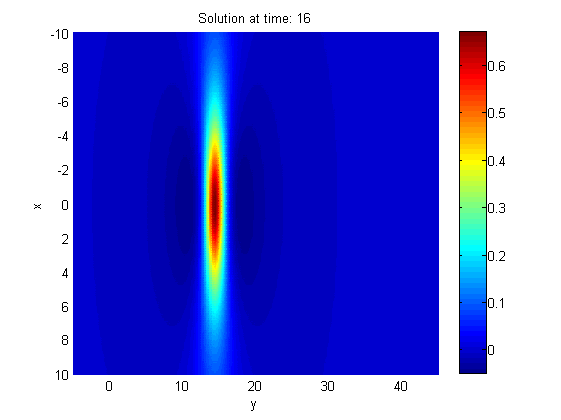
\includegraphics[width=\linewidth]{../amitans/figures/Solution1_t=16.png}
	\end{minipage}
	\begin{minipage}[b]{0.30\linewidth}
		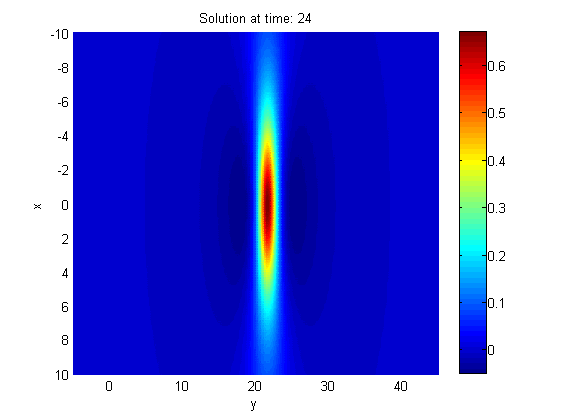
\includegraphics[width=\linewidth]{../amitans/figures/Solution1_t=24.png}
	\end{minipage}	
	\begin{minipage}[b]{0.30\linewidth}
		 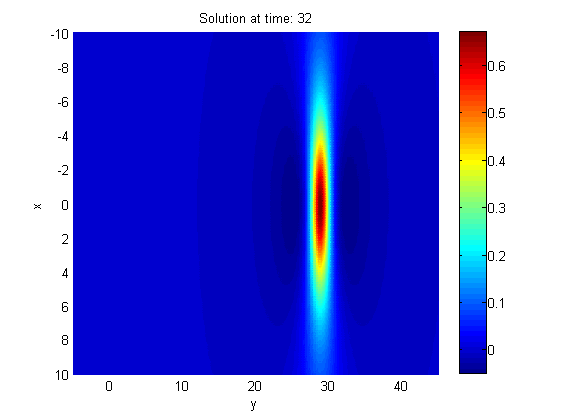
\includegraphics[width=\linewidth]{../amitans/figures/Solution1_t=32.png}
	\end{minipage}
	\begin{minipage}[b]{0.30\linewidth}
		 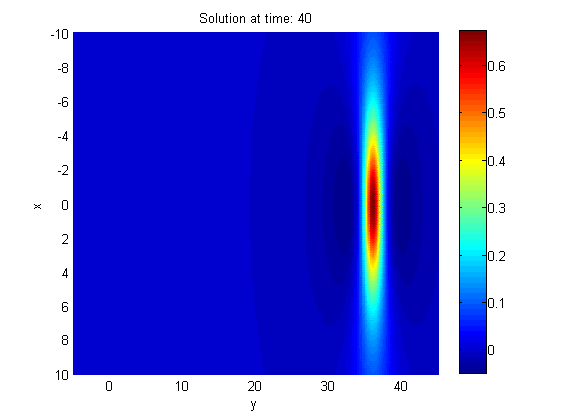
\includegraphics[width=\linewidth]{../amitans/figures/Solution1_t=40.png}
	\end{minipage}
\end{center}
Numerical solution of single wave for $\beta=1$ and $c = 0.9$ at times $t=0,8,16,24,32,40$.
\end{frame}

%------------------------------------------------------------------

\begin{frame}
\frametitle{Results}
\framesubtitle{Solution Maximum, Taylor Series, $O(|h|^6+\tau^6)$}

Two parameters sets are used:
\begin{description}
 \item[Test 3] $\beta = 3$, $c = 0.52$, $\Omega = [-40, 40] \times [-40, 60]$
 \item[Test 4] $\beta = 1$, $c = 0.9$, $\Omega = [-40, 40] \times [-80, 80]$
\end{description}
The end time is $T=40$ for both tests.
\begin{figure}[ht]
	\centering
	\begin{minipage}[b]{0.4\linewidth}
		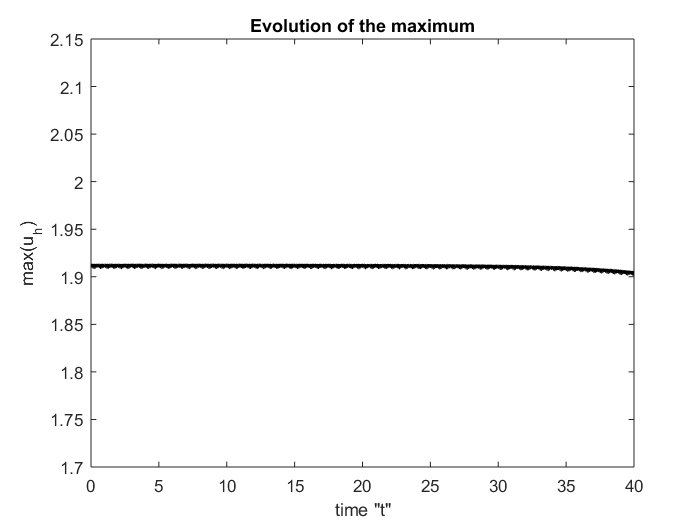
\includegraphics[width=\linewidth]{../amitans/figures/EvolutionOfMaximum_bt3_t40.png}
	\end{minipage}	
	\begin{minipage}[b]{0.4\linewidth}
		 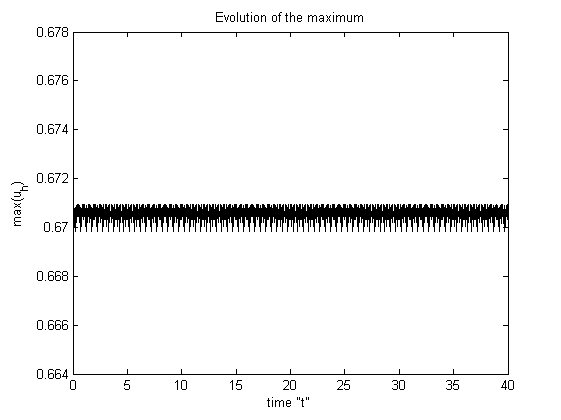
\includegraphics[width=\linewidth]{../amitans/figures/EvolutionOfMaximum_bt1_t40.png}
	\end{minipage}

Evolution of the maximum for Test Wave $\beta =3$ (left panel) and $\beta=1$ (right panel).
\end{figure}

\end{frame}

%------------------------------------------------------------------

\begin{frame}
\frametitle{Results}
\framesubtitle{Solution Shape, Taylor Series, $O(|h|^6+\tau^6)$}
\begin{figure}[ht]
	\centering
	\begin{minipage}[b]{0.49\linewidth}
		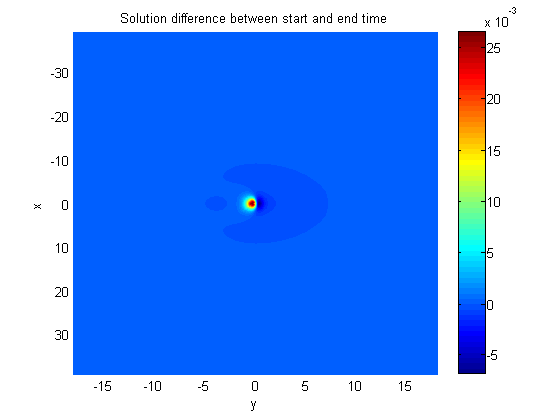
\includegraphics[width=\linewidth]{../amitans/figures/compare_start_end_bt3_c052.png}
	\end{minipage}	
	\begin{minipage}[b]{0.49\linewidth}
		 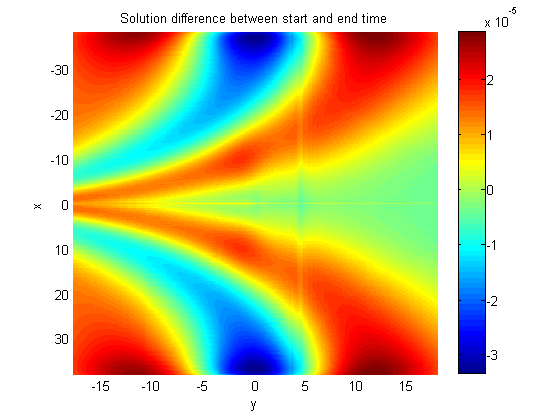
\includegraphics[width=\linewidth]{../amitans/figures/compare_start_end_bt1_c09.png}
	\end{minipage}

Difference between localized solitons at time $T=0$ and $T=40$ for Test 3 $\beta = 3$, $\beta = 0.52$  (left) and Test 4 $\beta=1$, $c=0.9$ (right). 
\end{figure}

It is obtained that:
\begin{description}
 \item[$\beta = 3$, $c = 0.52$] $||u_h(t=40)-u_h(t=0)|_{L_2} = 0.023453$
 \item[$\beta = 1$, $c = 0.9$] $||u_h(t=40)-u_h(t=0)|_{L_2} = 0.000812$
\end{description}
\end{frame}

%------------------------------------------------------------------


\begin{frame}
\frametitle{Mass for the TS method}

\begin{center}\vspace{0.4cm}
	\begin{minipage}[b]{0.49\linewidth}
		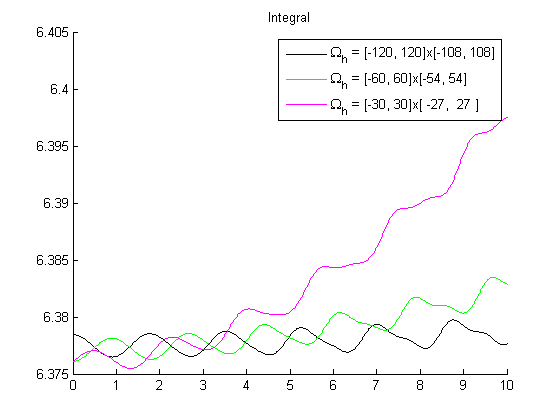
\includegraphics[width=\linewidth]{../amitans/figures/MassTaylor_120_60_30_ZB1_bt3_c045_h020_O(h^6).png}
	\end{minipage}	
	\begin{minipage}[b]{0.49\linewidth}
		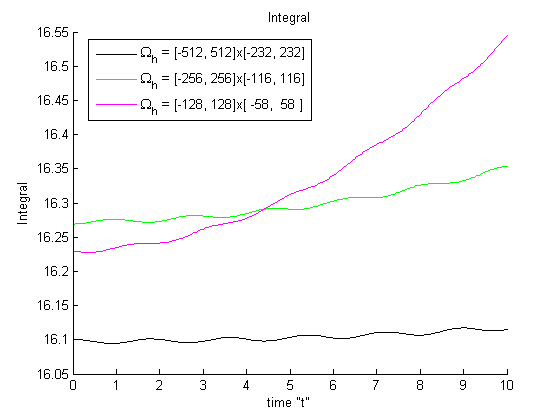
\includegraphics[width=\linewidth]{../amitans/figures/MassTaylor_512_256_128_ZB1_bt1_c090_h040_O(h^6).png}
		
	\end{minipage}
\end{center}
The Mass of the solution for approximation $O(|h|^6 + \tau^6)$ and $T = 10$ over three nested domains. Left panel is for Test 1 with $\beta=3$, $c = 0.45$ and right panel is for Test 2 with $\beta=1$, $c = 0.9$.
\end{frame}


\end{document}

